\pagebreak
\section{تراز کردن دنباله ژنتیکی\protect\footnote{\lr{sequence alignment}}}

\subsection*{مسئله بلندترین زیردنباله مشترک\protect\footnote{Longest Common Subsequence(LCS)}}

\begin{wrapfigure}{l}{6cm}
\centering
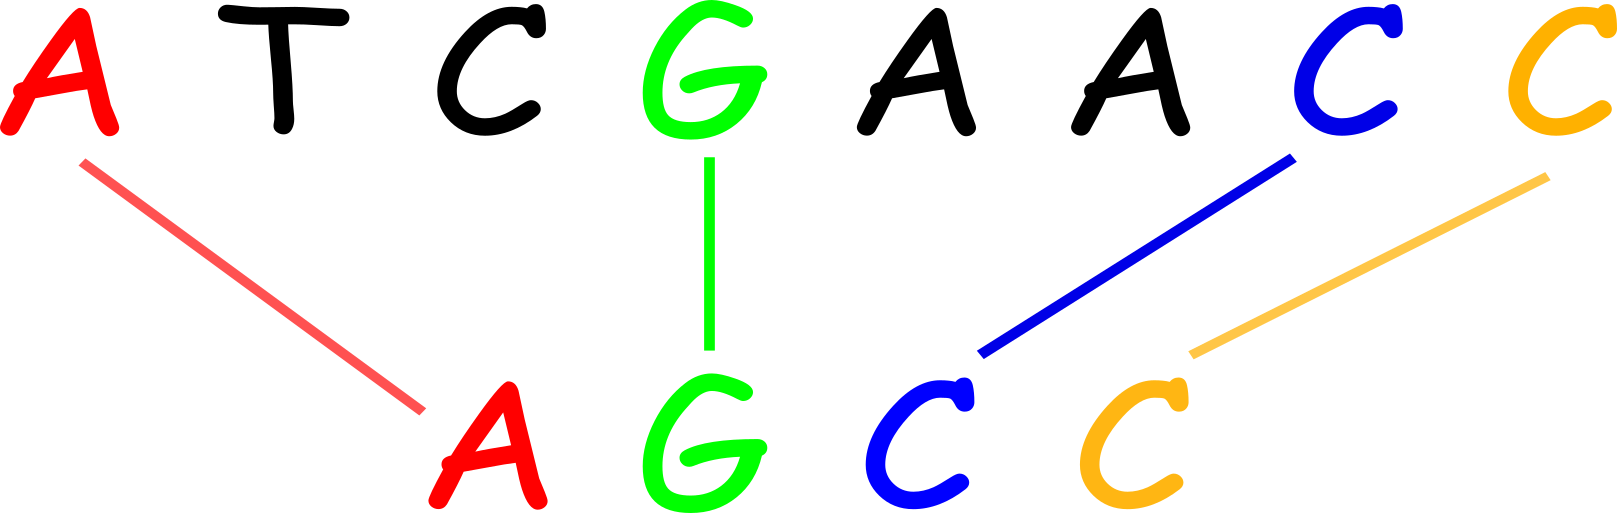
\includegraphics[width=6cm]{LCS1}
\caption{بلندترین زیردنباله مشترک}
\label{fig:lcs1}
\end{wrapfigure}

همانطور که در شکل
\ref{fig:lcs1}
مشاهده می‌کنید می‌خواهیم بلندترین زیردنباله از دو دنباله را پیدا کنیم. فرض کنید که
$Z$
یک زیر دنباله از دنباله
$ٓX$
باشد. حال می‌گوئیم که
$Z$
زیردنباله مشترک
\footnote{\lr{common subsequence}}
$A$
و
$B$
است اگر
$Z$
هم زیردنباله
$A$
باشد و هم زیردنباله
$B$.
حال مسئله را به صورت زیر بیان می‌کنیم:
\begin{itemize}
\item
ورودی: دنباله‌های 
$A$
و
$B$
\item
خروجی: بلندترین زیردنباله مشترک
$A$
و
$B$
\end{itemize}

دنباله
$X = n_{1}n_{2} ... n_{m}$
را درنظر بگیرید یک
\lr{Prefix}
از
$X$
را به صورت زیر تعریف می‌کنیم:
\[X_{i}=n_{1}n_{2} ... n_{m}~~~~~~1\leq i \leq m\]

دو دنباله
$X = x_{1}x_{2} ... x_{m}$
و
$Y = y_{1}y_{2} ... y_{n}$
را در نظر بگیرید. حال فرض کنید که
$Z = z_{1}z_{2} ... z_{k}$
بزرگترین زیردنباله از
$X$
و
$Y$
باشد. می‌خواهیم حالت‌های ممکن برای
$Z$
را با توجه به کاراکترهای آخر
$X$
و
$Y$
بررسی کنیم:
\begin{enumerate}
\item
$x_{m} = y_{n} $
در نتیجه
$Z_{k-1}$
بلندترین زیردنباله مشترک برای
$X_{m-1}$
و
$Y_{n-1}$
است.

\begin{itemize}
\item اثبات:
اگر
$x_{m} = y_{n} $
می‌توان نتیجه
گرفت:
$ z_{k} = x_{m} = y_{n}$
چرا که در غیر اینصورت
$z_{k}$
کاراکتری مشترک از
$X$
و
$Y$
است که قبل از
$x_{n}$
و
$y_{m}$
انتخاب شده است. در اینصورت می‌توان
$x_{m} = y_{n} $
به انتهای
$Z$
اضافه کرد و این با بلندترین دنباله بودن
$Z$
در نتاقض است.
در نتیجه
$Z_{k-1}$
بلندترین زیردنباله مشترک برای
$X_{m-1}$
و
$Y_{n-1}$
است.
\end{itemize}

\begin{figure}[htbp]
\centering
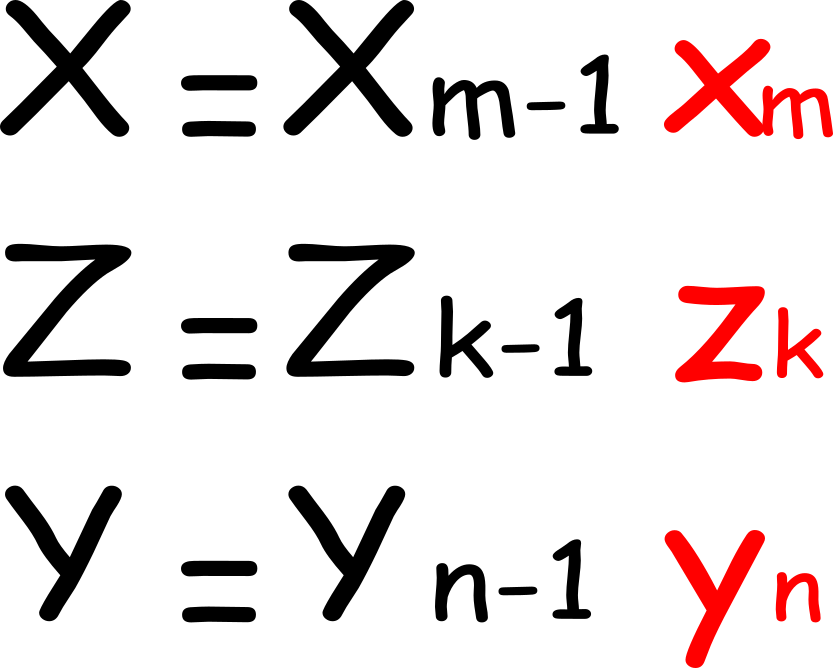
\includegraphics[width=2cm]{LCS2}
\end{figure}

\item
$x_{m} \neq y_{n}, z_{k} \neq x_{m}$
در نتیجه
$Z$
بلندترین زیردنباله مشترک
$Y_{n}$
و
$X_{m-1}$
است.
\item
$x_{m} \neq y_{n}, z_{k} \neq y_{n}$
در نتیجه
$Z$
بلندترین زیردنباله مشترک
$Y_{n-1}$
و
$X_{m}$
است.
\end{enumerate}

توجه شود که از مورد 2 و 3 ممکن است یک کدام و یا هر دو اتفاق بیافتد. حال به رابطه بازگشتی زیر می‌رسیم:
\[
  C_{i,j} =
    \begin{cases}
      0 & i=0 ~\text{or}~ j = 0\\
      C_{i-1,j-1} + 1 & i,j>0,x_{i}=y_{j}\\
      \max{\{C_{i-1,j}, C_{i,j-1}\}} & i,j>0,x_{i} \neq y_{j}
    \end{cases}  
\]

در نتیجه برای پیدا کردن
$C_{i,j}$
تنها کافی است که عضو بالایی، سمت چپ و چپ-بالا را داشته باشیم. حال با استفاده از
\lr{DP}
ردیف به ردیف از سمت چپ به راست،
$C_{i,j}$
ها را محاسبه می‌کنیم.

\unsetRL
\lr{
\begin{algorithm}
\caption{Longest Common Subsequence of X and Y}
\label{alg:LCS}
\begin{algorithmic}
\Require X and Y, two strings
\State $m = X.length$
\State $n = Y.length$
\State Initilize $ B[1 .. m, 1 .. n] $ and $C[0 .. m, 0 .. n]$
\ForEach {$i$ in $0, ..., m$  }
	\State $C_{i,0} = 0$
\EndFor
\ForEach {$j$ in $0, ..., n$  }
	\State $C_{0,j} = 0$
\EndFor
\ForEach {$i$ in $1, ..., m$  }
	\ForEach {$j$ in $1, ..., n$  }
		\If{$x_{i}=y{j}$}
			\State $C_{i,j} = C_{i-1,j-1} + 1$
			\State $B_{i,j} = `\nwarrow$'	
		\ElsIf{$C_{i-1,j}\geq C_{i,j-1}$}	
			\State $C_{i,j} = C_{i-1,j}$
			\State $B_{i,j} = `\leftarrow$'	
		\Else	
			\State $C_{i,j} = C_{i,j-1}$
			\State $B_{i,j} = `\uparrow$'
		\EndIf
	\EndFor
\EndFor
\State return $B$ and $C$
\end{algorithmic}
\end{algorithm}
}
\setRL


\unsetRL
\lr{
\begin{algorithm}
\caption{Print Longest Common Subsequence}
\label{alg:printLCS}
\begin{algorithmic}
\Require X, B, i, j
\If{$i=0$ or $j=0$}
	\State return	
\ElsIf{$B_{i,j} = `\nwarrow$'}	
	\State repeat algorithm for X, B, i-1, j-1
	\State print $X_{i}$	
\ElsIf{$B_{i,j} = `\uparrow$'}	
	\State repeat algorithm for X, B, i-1, j
\ElsIf{$B_{i,j} = `\leftarrow$'}	
	\State repeat algorithm for X, B, i, j-1
\EndIf
\end{algorithmic}
\end{algorithm}
}
\setRL

\pagebreak
مرتبه الگوریتم
\ref{alg:LCS}
از
$O(n \times m)$
است.

\begin{figure}[htbp]
\centering
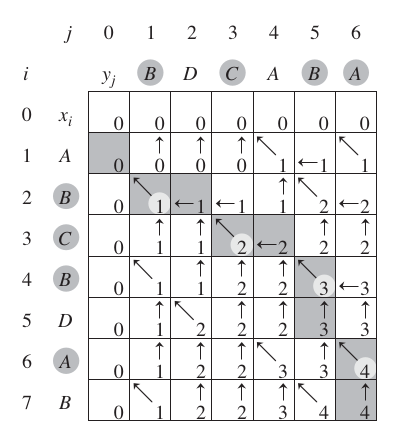
\includegraphics[width=7cm]{LCSTable}
\end{figure}